\chapter{Arquitectura de apilamiento PC/104}\label{cap:pc104}

Este capítulo estudia el formato PC/104, que se usa como estándar para apilar placas dentro de un CubeSat. El objetivo es obtener las dimensiones de la placa, los agujeros de fijación, los conectores y los pines que condicionan el diseño del PCB del transponder.

\section{El estándar PC/104 y su rol en los CubeSat}\label{sec:pc104-general}

PC/104 es una familia de estándares para computadoras embebidas, definidos por el PC/104 Embedded Consortium, que especifican tanto un factor de forma como un bus. El bus ISA (\emph{Industry Standard Architecture}) original combinaba dos buses de datos: el PC (8 bits) de 64 pines, que maneja señales de datos, y el PC/AT (16 bits) de 40 pines, que suma más lineas de interrupción y DMA\@. La suma de los pines da 104, lo que le da el nombre a la familia de estándares~\cite{pc104v24,pc104wiki}. 

Su principal característica es el apilamiento: los módulos se montan unos sobre otros mediante un conector de bus que atraviesa la placa y separadores en las cuatro esquinas, sin necesidad de \emph{backplane} (placa base común)~\cite{pc104v24}.

\begin{figure}[H]
  \centering
  \begin{subfigure}[t]{0.48\textwidth}
    \centering
    \fbox{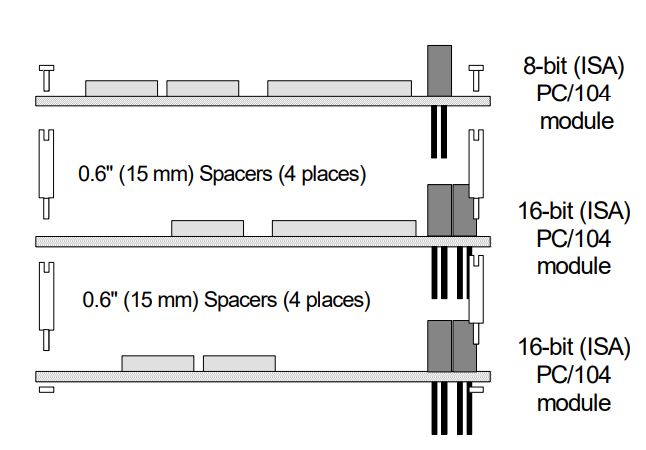
\includegraphics[width=\textwidth]{apilamiento.png}}
    \caption{}\label{fig:apilamiento-a}
  \end{subfigure}\hfill
  \begin{subfigure}[t]{0.48\textwidth}
    \centering
    \fbox{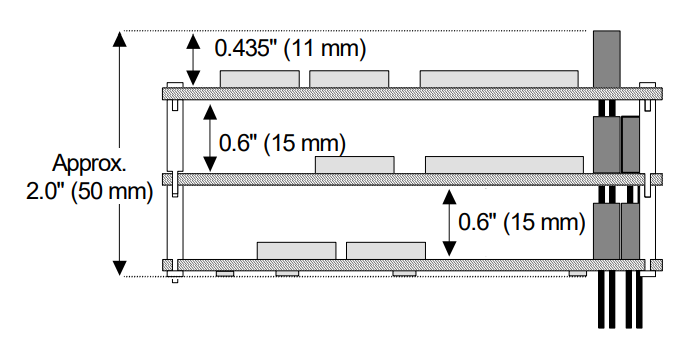
\includegraphics[width=\textwidth]{apilamiento2.png}}
    \caption{}\label{fig:apilamiento-b}
  \end{subfigure}
  \caption{Apilamiento de módulos típico. Fuente:~\cite[Sec. 2.2]{pc104v24}.}\label{fig:apilamiento}
\end{figure}


\subsection{Factor de forma frente a bus}\label{subsec:pc104-formafactor}

La especificación PC/104 define como obediente (\emph{compliant}) a los dispositivos que cumplen todos los aspectos no opcionales, sean mecánicos o eléctricos, y como \emph{bus-compatible} a los que no respetan las dimensiones pero proveen un conector de bus que sí cumple la especificación~\cite[Sec.~4]{pc104v24}. En el ámbito CubeSat, la tienda CubeSatShop aclara que la mayoría de los productos son <<bus-compatible>>: algunas especificaciones difieren levemente del estándar (como la posición del conector).

Cuando se habla de que un CubeSat usa PC/104, en la práctica se refiere a la forma de la placa, la ubicación de los agujeros de montaje y el conector físico de $2\times 2\times 26$ pines. Los CubeSats no adoptan la señalización ni los protocolos del estándar PC/104, y la asignación de cada pin queda a criterio del fabricante~\cite{cubesatshopfaq}. 

Un mensaje en una lista de correo de AMSAT ilustra el problema desde el lado del diseñador los conectores ocupan espacio, y no siempre se usa la cantidad completa de pines, además de que agregan masa de un solo lado, lo que desplaza el centro de masa. Señala también que los diseños de AMSAT usan varios buses a la vez (RS232, I2C, CAN y señales discretas), con interfaces, tensiones y firmware distintos~\cite{amsatpc104}. 

La propia CDS no menciona el PC/104 en su texto; es una convención de la industria, y no un requisito de lanzamiento.

%--------------------------------------------------------------------
\section{Dimensiones geométricas y orificios de fijación}\label{sec:pc104-dimensiones}

Las Figuras~\ref{fig:pc104-dim-16} y~\ref{fig:pc104-dim-8} resume la geometría del módulo según el Apéndice~A de la especificación PC/104 v2.4~\cite{pc104v24}. Las versiones de 8 y 16 bits tienen el mismo patrón de agujeros desde la versión 2.1 de la especificación~\cite{pc104v24}.

\begin{figure}[H]
  \centering
  \fbox{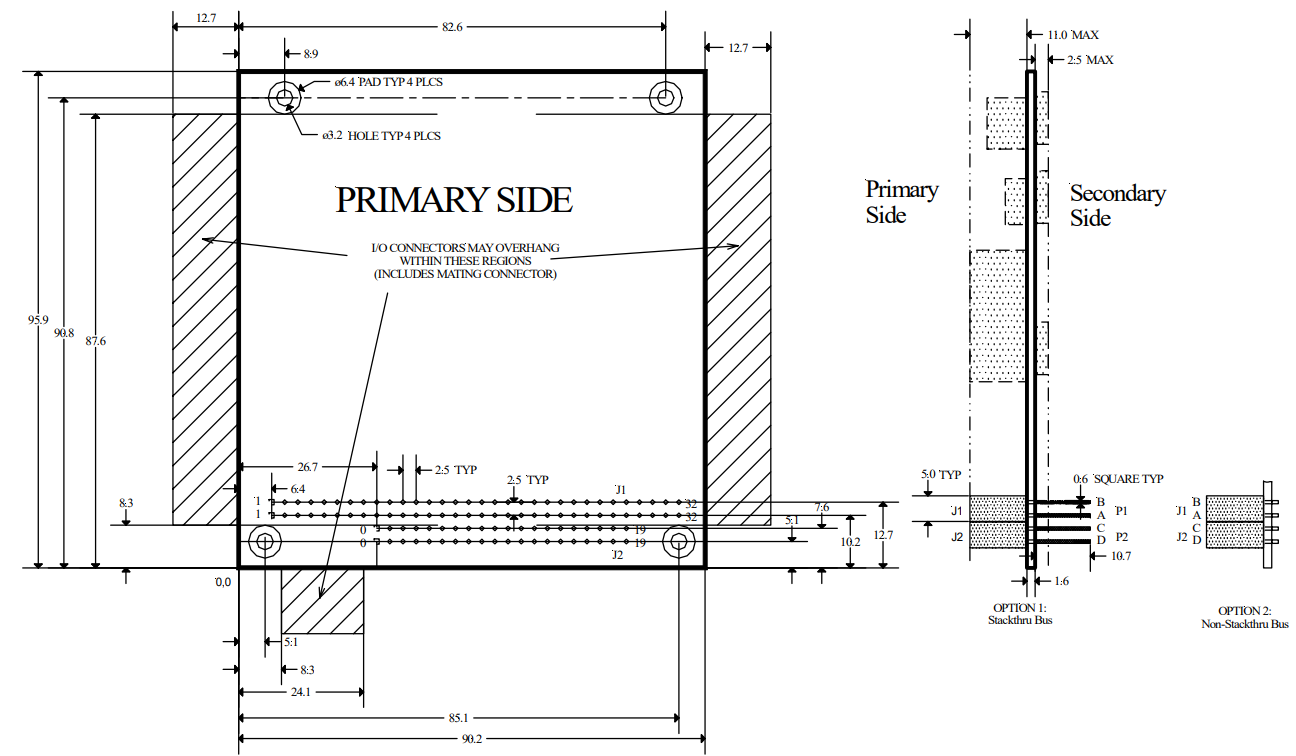
\includegraphics[width=0.98\textwidth]{pc104_dim_16.png}}
  \caption{Dimensiones de módulo de PC/104 16-bit en milímetros.}\label{fig:pc104-dim-16}
\end{figure}

\begin{figure}[H]
  \centering
  \fbox{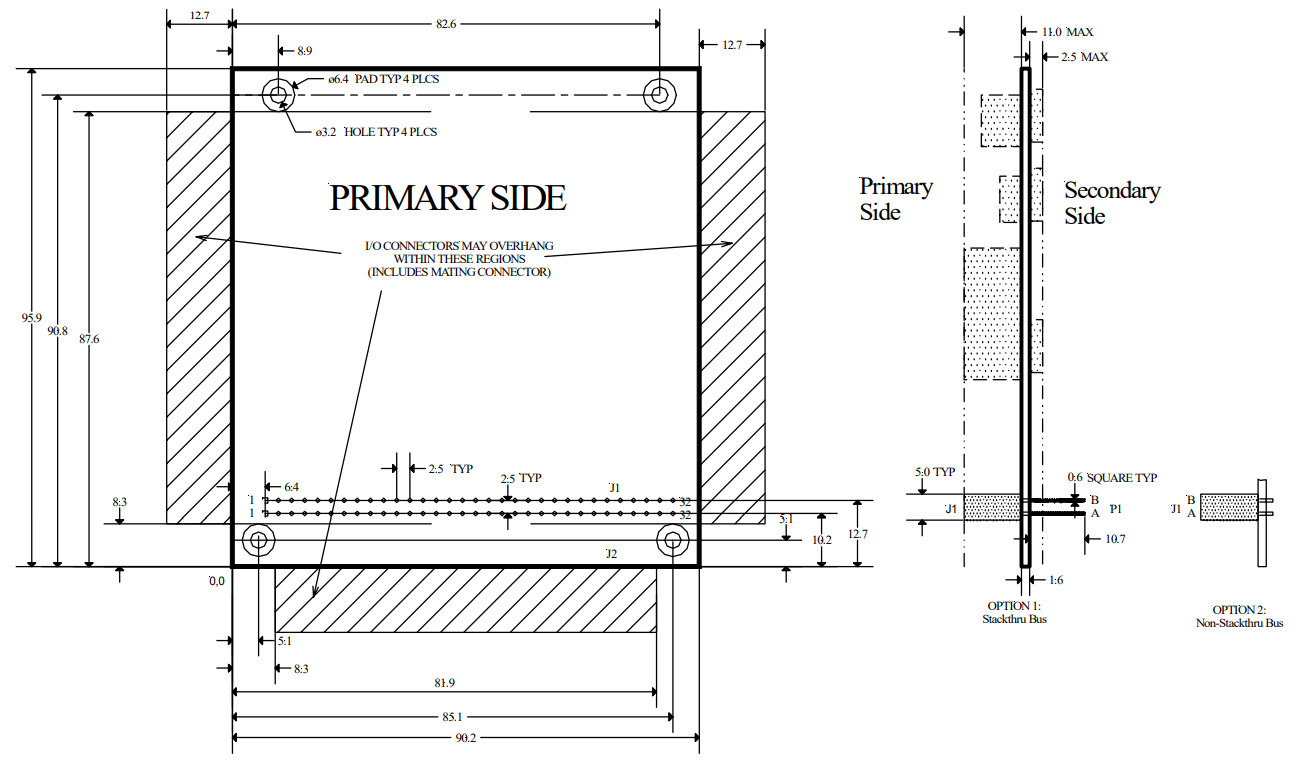
\includegraphics[width=0.98\textwidth]{pc104_dim_8.png}}
  \caption{Dimensiones de módulo de PC/104 8-bit en milímetros.}\label{fig:pc104-dim-8}
\end{figure}

La especificación ofrece dos opciones de bus según si los conectores P1 y P2 atraviesan el módulo (\emph{stackthrough}) o no. Si se combinan módulos de 8 y 16 bits en una pila, los de 16 bits deben ir por debajo de los de 8 bits, como puede observarse en la Figura~\ref{fig:apilamiento}~\cite[Sec.~2.2]{pc104v24}.

\subsection{Variaciones en placas para CubeSat}\label{subsec:pc104-variaciones}

Las placas comerciales para CubeSat respetan el patrón de agujeros, pero el contorno varía levemente entre fabricantes. La Tabla~\ref{tab:ejemplos} compara dos placas de prototipado de empresas distintas, aunque ambas son compatibles con los agujeros de fijación y la ubicación de los conectores~\cite{pumpkinprotoboard,ardusat}.

\begin{table}[H]
  \centering
  \begin{tabular}{@{}llccc@{}}
    \toprule
    Empresa & Modelo & Ancho [\si{\milli\metre}] & Largo [\si{\milli\metre}] & Masa [\si{\gram}] \\
    \midrule
    Pumpkin & Prototyping / Breadboard Module & \num{96} & \num{90} & \num{43}~\cite{pumpkinprotoboard} \\
    ArduSat & Prototyping Module & \num{95,45} & \num{90,3} & \num{42}~\cite{ardusat} \\
    \bottomrule
  \end{tabular}
  \caption{Dimensiones y masa de placas de prototipado comerciales para CubeSat.}\label{tab:ejemplos}
\end{table}

También se tienen alturas máximas por sobre y por debajo de la placa, lo cual tiene consecuencias de diseño: la altura máxima de componentes están acotados, tanto por la separación de la pila como por la altura de los conectores. Los valores concretos dependen del fabricante del resto de la pila y deben acordarse con el equipo que arma el satélite.

%-------------------------------------------------
\section{Conectores}\label{sec:pc104-conectores}

\subsection{Conector PC/104 original}\label{subsec:pc104-conector-orig}

El bus PC/104 tiene dos conectores: P1/J1, de 64 pines (2 filas de 32: A y B), y P2/J2, de 40 pines (2 filas de 20: C y D), que suman las 104 conexiones del nombre~\cite[Sec.~1 y Apéndice~B]{pc104v24}. Los módulos de 8 bits solo necesitan el conector P1. La Tabla~\ref{tab:pc104-conector-esp} resume las especificaciones del conector del Apéndice~D de la especificación.

\begin{table}[H]
  \centering
  \begin{tabular}{@{}>{\raggedright\arraybackslash}p{5.5cm}>{\raggedright\arraybackslash}p{9cm}@{}}
    \toprule
    Parámetro & Característica \\
    \midrule
    Capacidad de corriente & \SI{1}{\ampere} continuo por pin \\
    Resistencia de contacto & $<\SI{30}{\milli\ohm}$ \\
    Rigidez dieléctrica & \SI{1000}{\volt} (CA) \\
    Resistencia de aislación & $\geq \SI{5000}{\mega\ohm}$ \\
    Temperatura de operación & de \SI{-55}{\celsius} a \SI{+85}{\celsius} \\
    Durabilidad & 50 ciclos mínimo \\
    Carcasa & Termoplástico de alta temperatura, UL 94-V0 \\
    Contacto & Bronce fosforoso \\
    \bottomrule
  \end{tabular}
  \caption{Especificaciones del conector de bus PC/104 (v2.4, Apéndice~D).}\label{tab:pc104-conector-esp}
\end{table}

\subsection{Conector del CubeSat Kit Bus}\label{subsec:pc104-cskb}

En los CubeSats se usa un conector propio, el \emph{CubeSat Kit Bus} (CSKB), que consiste en dos conectores, H1 y H2, de $2\times2\times 26$ pines cada uno (104 pines en total), ubicados en el mismo lugar que los conectores PC/104 sobre la placa~\cite{pumpkinmb,cubesatshopfaq,amsatpc104}.
Pumpkin especifica una corriente máxima de \SI{3}{\ampere} por pin del conector CSKB~\cite{pumpkinmb}, frente a \SI{1}{\ampere} del conector PC/104 original (Tabla~\ref{tab:pc104-conector-esp}).

%--------------------------------------------------------------------
\section{Distribución de pines}\label{sec:pc104-pines}

Las señales del PC/104 original son idénticas a las del bus ISA, las únicas que importan son las de alimentación y masa.

La asignación de pines de H1 y H2 no forma parte de ningún estándar formal: es la convención de Pumpkin, que otros fabricantes siguieron con variantes~\cite{amsatpc104}. Por ejemplo, la hoja de opciones de la computadora a bordo CubeComputer (CubeSpace) permite configurar algunos pines (bus I2C secundario en H1.21 y H1.23, alimentación de 3,3\,V siempre activa en H2.27 y H2.28)~\cite{cubespace}. 

La Sección \emph{CubeSat Kit Bus PIN DESCRIPTIONS} de la hoja del datos del modelo \emph{Single Board Computer Development Platform} de Pumpkin muestra la función de cada uno de los pines del conector~\cite{}.

% Haceme una cita de esto si no está: https://www.pumpkininc.com/space/datasheet/710-00297-E_DS_DB.pdf
